\section{The Real Numbers}
\subsection{Construction of the Real Numbers}
\label{sec:costruzione_reali}

The property that the field $\QQ$ of rational numbers lacks is
\emph{continuity}. It is not sufficient to add a new operation; rather, it is
necessary to ensure that every pair of separated sets has a separation element
(see definition~\ref{def:ordinamento_continuo}), meaning that every non-empty
and upper-bounded set must have a least upper bound.

We can then define the set of \emph{real numbers} as follows:
\index{real!set of}%
\index{number!real}%
\index{set!real numbers}%
\[
\RR = \ENCLOSE{A \in \mathcal P(\QQ)\colon A\neq \emptyset, \text{ $A$ upper bounded}}/\sim
\]
where we set $A\sim B$ if $A$ and $B$ have the same upper bounds, that is, if
for every $q\in \QQ$, $q\ge A \iff q\ge B$. The idea behind this definition is
that real numbers can be identified by their lower approximations through
rational numbers. However, different approximations can represent the same real
number.

\begin{exercise}
  Show that $A \sim B \sim C$ for the following sets:
  \[
  A = \ENCLOSE{1}, \qquad 
  B = \ENCLOSE{x\in \QQ\colon x<1}, \qquad
  C = \ENCLOSE{\frac{n}{n+1}\colon n\in \NN}.
  \]
\end{exercise}

\begin{exercise}
  Show that $A\sim B$ if
  \[
  A = \ENCLOSE{x\in \QQ\colon x^2<2}, \qquad
    B = \ENCLOSE{\frac{n}{10^k}\colon n\in \NN, k\in \NN, n^2 \le 2\cdot 100^k <
  (n+1)^2}.
  \]
  Verify that 
  \[
    B \supset \ENCLOSE{
      1,\frac{14}{10},\frac{141}{100},\frac{1414}{1000},
      \frac{14142}{10000}}.
  \]
\end{exercise}

We now wish to define an ordered group structure on $\RR$.

The ordering of $\QQ$ can be easily extended to $\RR$ by defining
$\Enclose{A}_\sim \le \Enclose{B}_\sim$ if every upper bound of $B$ is also an
upper bound of $A$. This definition does not depend on the choice of $A$ and $B$
within their equivalence class because within the equivalence class, the set of
upper bounds does not change.

For addition, given $A,B$ non-empty and upper-bounded subsets of $\QQ$, we
define
\[
  \Enclose{A}_\sim+\Enclose{B}_\sim
  = \Enclose{A+B}_\sim
  \qquad\text{where $A+B = \ENCLOSE{a+b\colon a \in A, b \in B}$.}
\]
Clearly, $A+B$ is non-empty and upper-bounded, and it is not difficult to prove
that if $A\sim A'$ and $B\sim B'$, then $A+B\sim A'+B'$.

\begin{theorem}
  \label{th:reali_gruppo_continuo}%
With the addition and ordering just defined, $\RR$ turns out to be a totally
ordered, dense, and continuous additive group
(definitions~\ref{def:ordinamento_denso}, \ref{def:gruppo_ordinato},
\ref{def:ordinamento_continuo}).
\end{theorem}
\begin{proof}
    Clearly, $x\le x$, if $x\le y$ and $y\le x$, then $x=y$, and if $x\le y$,
  $y\le z$, then $x\le z$: thus, $\le$ is an ordering on $\RR$. It is also a
  total ordering because given $x=\Enclose{A}_\sim$ and $y=\Enclose{B}_\sim$, if
  $x\neq y$, it means that the set of upper bounds of $A$ is different from the
  set of upper bounds of $B$. Suppose then that there exists $q$ that is an
  upper bound of $A$ but not an upper bound of $B$ (if the reverse happens, just
  swap $A$ and $B$). In such a case, $B\ge A$ since every upper bound of $B$
  must be greater than $q$ and therefore must also be an upper bound of $A$,
  from which $x\le y$.
  
    Obviously, addition on $\RR$ is associative and commutative since these
  properties hold on $\QQ$ and consequently on its subsets: $(A+B)+C = \{
  a+b+c\colon a\in A, b\in B, c\in C\} = A + (B+C)$ and $A+B = \{a+b\colon a\in
  A, b\in B\} = B+A$. Since $A+\ENCLOSE{0} = A$, we also note that
  $\Enclose{\ENCLOSE{0}}_\sim$ is the neutral element of addition.
  
    Given $A\in \mathcal R$, we denote by $A'$ the set of upper bounds of $A$.
  We want to prove that $A$ and $A'$ contain arbitrarily close points:
  \begin{equation}\label{eq:48023775}
  \forall \eps\in\QQ\colon (\eps >0 \implies \exists a \in A\colon \exists b\in A'\colon
  b-a < \eps).
  \end{equation}
    To do this, take any $c\in A$ and take any $q\in A'$ ($A\neq \emptyset$ and
  since $A$ is upper-bounded, $A'\neq \emptyset$). The set $I=\ENCLOSE{n\in \NN
  \colon c+n\eps\in A'}$ is not empty because if $n>\frac{q-c}\eps$, then
  $c+n\eps>q$, and since $q$ is an upper bound of $A$, $c+n\eps$ is also an
  upper bound. Thus, by the well-ordering principle of $\NN$
  (theorem~\ref{th:buon_ordinamento}), the set $I$ has a minimum, which we call
  $k$. If $k=0$, it means that $c\in A'$, and setting $a=b=c$,
  \eqref{eq:48023775} is trivially satisfied. Otherwise, take $b=c+k\eps$. By
  the choice of $k$, we know that $b\in A'$ and $c+(k-1)\eps$ is not an upper
  bound of $A$. But then there exists $a\in A$ such that $a>c+(k-1)\eps$, from
  which $b-a < \eps$, and \eqref{eq:48023775} is still satisfied.
  
    We can now observe that setting $B=-A' = \{-x\in \QQ \colon x$ is an upper
  bound of $A\}$, we have $(A+B)\sim\ENCLOSE{0}$. The upper bounds of
  $\ENCLOSE{0}$ are the $q\in \QQ$ with $q\ge 0$. We want to prove that $A+B$
  also has the same upper bounds. But if $a\in A$ and $b\in B$, it results that
  $-b\ge a$, i.e., $a+b\le 0$, so $0$ is an upper bound of $A+B$, and any $q\ge
  0$ is even more so. If instead $q<0$, by property \eqref{eq:48023775}, there
  exist $a\in A$ and $-b\in A'$ (i.e., $b\in B$) such that $(-b)-a<-q$, i.e.,
  $a+b>q$. Thus, $q<0$ is not an upper bound of $A+B$, and we conclude that
  $A+B\sim\ENCLOSE{0}$.
  
    This proves that given any $x\in \RR$, if $x=\Enclose{A}_\sim$, setting
  $y=\Enclose{-A'}$, we have $x+y=\Enclose{0}_\sim$. Thus, every $x\in \RR$ has
  an opposite $y$, which we will denote by $y=-x$.

    The ordering is compatible with addition because if $\Enclose{A}_\sim \le
  \Enclose{B}_\sim$ and $A,B,C\in \mathcal R$, then if $q$ is an upper bound of
  $B+C$, for every $c\in C$, $q-c$ is an upper bound of $B$, and thus $q-c$ is
  also an upper bound of $A$. But then $q$ is an upper bound of $A+C$. Thus, if
  $x\le y$ and $x,y,z\in \RR$, we have $x+z\le y+z$, and $\RR$ is an ordered
  group.
  
    The ordering of $\RR$ is dense (definition~\ref{def:ordinamento_denso}).
  Indeed, if $x<y$, setting $y-x=\Enclose{A}_\sim$, we know that every upper
  bound of $A$ is greater than or equal to $0$. But if every positive number
  were an upper bound of $A$, we would have $A\sim\ENCLOSE 0$, which is not
  possible since $x\neq y$. Thus, there exists $q>0$ that is not an upper bound
  of $A$. But then $y-x \ge \Enclose{\ENCLOSE q}_\sim > \Enclose{\ENCLOSE{\frac
  q 2}}_\sim = \eps > 0$, from which $x<x+\eps<y$.
  
    We now prove that the ordering is continuous. Let $\mathcal A$ and $\mathcal
  B$ be non-empty subsets of $\RR$ with $\mathcal A\le \mathcal B$. We can
  define
  \begin{align*}
        C & = \bigcup\ENCLOSE{A\in \mathcal P(\QQ)\colon \Enclose{A}_\sim \in
    \mathcal A} \\
      &= \ENCLOSE{q\in \QQ\colon \exists A\colon 
      (\Enclose{A}_\sim \in \mathcal A) \land (q\in A)}.
  \end{align*}
    For any $a=\Enclose{A}_\sim \in \mathcal A$, it is obviously $A\subset C$.
  In particular, $C$ is not empty. While if $b=\Enclose{B}_\sim \in \mathcal B$,
  for any $q\in C$, $q\in A$ for some $A$ such that $\Enclose{A}_\sim = a\in
  \mathcal A$. But since $a\le b$, every upper bound of $B$ is also an upper
  bound of $A$. In particular, for any $r$ that is an upper bound of $B$, $r$ is
  an upper bound of $C$. Then $C$ is non-empty and upper-bounded, and setting
  $c=\Enclose{C}_\sim$, it results that every upper bound of $C$ is an upper
  bound of every $A$ with $\Enclose{A}_\sim \in \mathcal A$, while every upper
  bound of any $B$ with $\Enclose{B}_\sim\in \mathcal B$ is also an upper bound
  of $C$. This means that $c\ge a$ for every $a\in A$ and $b\ge c$ for every
  $b\in B$: the proof is concluded.
\end{proof}

To each $q\in \QQ$, we can associate the element $\Enclose{\ENCLOSE q}_\sim$ of
$\RR$. Obviously, if $q\neq s$ in $\QQ$, then $\ENCLOSE{q}$ and $\ENCLOSE{s}$ do
not have the same upper bounds, and thus distinct elements of $\RR$ are
obtained. Moreover, given $x<y$ in $\RR$, we can always find $q\in \QQ$ such
that $x < \Enclose{\ENCLOSE q}_\sim < y$. If $x=\Enclose{A}_\sim$ and
$y=\Enclose{B}_\sim$, it suffices to take an upper bound $m\in \QQ$ of $A$ that
is not an upper bound of $B$ and an element $M>m$ of $B$ and choose $q$ such
that $m<q<M$.

By identifying $q$ with $\Enclose{\ENCLOSE q}_\sim$, we can thus think that $\QQ
\subset \RR$, and it follows that $\QQ$ is dense in $\RR$, and consequently,
$\RR$ is itself dense.

Just as we extended addition from $\QQ$ to $\RR$, we could easily extend the
multiplication operation as well.
% We will only need to be careful that multiplication by a negative number reverses the ordering and thus swaps upper bounds with lower bounds.
% 
% Given $x\in \RR$ and $y\in \RR$, $y \ge 0$, we will have $x=[A]_\sim$ and $y=[B]_\sim$ for some $A,B$ non-empty and upper-bounded subsets of $\QQ$. We could then define:
% \[
%   y\cdot x = [A\cdot B]_\sim
% \]  
% where $A\cdot B$ is the set of all products $a\cdot b$ with $a\in A$ and $b\in B$.
However, we will not need to define multiplication now; we will obtain it later
through a more general construction (theorem~\ref{th:moltiplicazione_reali}).

\subsection{Uniqueness of the Real Numbers}

In the previous chapter, we constructed a set $\RR$ that turns out to be a
totally ordered, dense, and continuous additive group. In this chapter, we want
to prove (theorem~\ref{th:isomorfismo}) that $\RR$ is essentially the only group
that satisfies such properties, in the sense that every totally ordered, dense,
continuous, and non-trivial additive group is isomorphic to $\RR$.

% There exist additive groups that extend $\RR$, but no extension maintains all the properties of the ordering of $\RR$. The \emph{complex} numbers (which we will see shortly) and the \emph{quaternions}, for example, are not totally ordered. The \emph{hyperreal} numbers of Robinson, which form the basis of non-standard analysis, do not satisfy the continuity property of the ordering. The same holds for the \emph{surreal} numbers introduced by Conway.

We therefore want to consider a generic additive group $R$. We will also assume
that $R$ is non-trivial, meaning that the group does not consist solely of the
neutral element: $R\neq \ENCLOSE{0}$.

In fact, the properties of $R$ correspond exactly to the properties we expect a
geometric line to have: the ordering corresponds to the property that each point
on the line divides the line into two parts and that given any two points,
intermediate points can be identified. The addition operation corresponds to the
ability to perform translations along the line.

% Intuitively, the set $\RR$ of real numbers can be obtained from a geometric line in the same way a ruler is constructed. We start by marking a reference point on the line, which we call $0$, and then observe that the point $0$ (like any other point) divides the line into two parts. Arbitrarily, we call positive the points on one side and negative the points on the other side. On the half-line of positive numbers, we arbitrarily choose a point $1$. The segment between the points $0$ and $1$ will be our unit of measure. Addition could be defined using rigid movements. Translating the point $1$ one unit at a time, we obtain, by iteration, all natural numbers. Translating backward, we obtain negative integers. Assuming that between any two points there are always intermediate points (divisibility) and assuming that dividing the line into two parts always results in a division point (continuity), we will show how to divide any segment into $n$ equal parts for any natural number $n$. In this way, we will rediscover rational numbers and multiplication by a rational number. With a growing extension, we will then be able to define multiplication between real numbers. We will then observe that the multiplicative structure of positive real numbers satisfies the same axioms as the additive structure of reals, and thus the construction made to build multiplication can be repeated identically to build exponentiation.

\begin{theorem}[Archimedean Property]
  \label{th:archimede}%
  \mymark{**}%
  \mymargin{Archimedean property}%
  \index{property!Archimedean}%
  \mynote{This theorem tells us that the group $R$ contains neither \emph{infinite} elements (i.e., larger than any multiple of a positive number $x$) nor \emph{infinitesimal} elements (i.e., smaller than any fraction $\frac{x}{n}$ with $x>0$ and $n\in \NN$). Thus, the infinitesimal quantities used by Newton and Leibniz to define derivatives and integrals are not justifiable within a totally ordered, dense, and continuous group. However, it is possible to define a totally ordered, dense, but not continuous group in which infinite and infinitesimal quantities exist: this is what is done in \emph{non-standard analysis}. \index{non-standard analysis}%
  }
        Let $R$ be a totally ordered, dense, and continuous group. Then for
    every $x,y\in R$, $x>0$, $y>0$, there exists $n\in \NN$ such that $n\cdot x
    > y$.
\end{theorem}
%
\begin{proof}
\mymark{*}%
Fix $x>0$ and consider the sets:
\[
A = \NN\cdot x = \ENCLOSE{n\cdot x\colon n\in \NN}, \qquad
B = \ENCLOSE{b\in R\colon \forall n\in\NN\colon n \cdot x \le b }.
\]
By definition, $A\le B$, and $A$ is non-empty. If, for the sake of
contradiction, the theorem were false, we would have $y\in B$, and thus $B$
would also be non-empty. Therefore, by the continuity of the ordering, there
should exist a separation element $s\in R$ such that $A\le s\le B$. Since
$s-x<s$ and $s\le B$, we know that $s-x \not \in B$. Thus, there exists $n\in
\NN$ such that $n\cdot x > s-x$, but then $(n+1)\cdot x > s-x+x=s$. But this is
absurd because $(n+1)\cdot x\in A$ and $s\ge A$.
%
%%% proof with SUP
%  Fix $x,y\in R$, $x,y>0$ and consider the set 
%  \[
%     A = \NN \cdot y = \ENCLOSE{n\cdot y\colon n\in \NN}.
%  \]
%  It suffices to prove that $A$ is not upper-bounded because 
%  in that case, given $x\in \RR$, there would exist $n\in \NN$ such that $n\cdot y> x$.
%
%  Clearly, $A$ is not empty since $0\in A$, so if $A$ 
%  were upper-bounded, there would exist 
%  $m=\sup A$, $m\in R$. 
%  Since $m$ is the minimum of the upper bounds of $A$
%  and $m-y$ is smaller than $m$, then $m-y$ is not an upper bound. 
%  Therefore, there must exist $n\in \NN$ such that $ny>m-y$.
%  But then $(n+1)y = ny + y > m$, and since $n+1\in \NN$, we find that $m$
%  could not have been an upper bound of $A$: absurd.
\end{proof}

If $n\cdot x = y$ and $n\neq 0$, we will write $x=\frac y n$. However, to ensure
this definition is unique, we need to verify that if $n\cdot x = n\cdot x'$,
then $x=x'$. Indeed, we have
\[
  0 = n\cdot x - n\cdot x' = n\cdot (x-x')
\]
and if $n\neq 0$, we conclude $x-x'=0$, i.e., $x=x'$.

The following theorem allows us to prove that division by $n\neq 0$ can always
be performed. Note that if we interpret this theorem on a multiplicative group
instead of an additive one, the result appears less trivial because we are
proving the existence of the $n$-th root.

\begin{theorem}[Divisibility]
\label{th:divisibile}%
If $R$ is a totally ordered, dense, and continuous additive group, then for
every $y\in R$ and for every $n\in \NN$, $n\neq 0$, there exists $x\in R$ such
that $n\cdot x = y$.
\end{theorem}
%
To prove the theorem, we will need the following lemma.
%
\begin{lemma}[Existence of Small Numbers]
  \label{lm:numeri_piccoli}%
Let $R$ be a totally ordered and dense additive group. For every $y\in R$,
$y>0$, and every $n\in \NN$, there exists $x\in R$, $x>0$, such that $nx\le y$.
\end{lemma}
%
\begin{proof}
We want to first prove that 
\begin{equation}\label{eq:41095633}
  \forall y>0 \colon \exists x>0 \colon x+x \le y.
\end{equation}
By the density property, we know that there exists $z$ such that $0<z<y$. Take
$w=y-z$. If $w\le z$, then $w+w\le w+z=y$, and we can take $x=w$. Otherwise,
$z+z < w+z = y$, and we can take $x=z$.
%% Note: the proof is delicate if the group is not commutative: attention must be paid to the order of the addends!

Consider now the set $M$ of natural numbers that satisfy the theorem:
\[
  M \defeq \ENCLOSE{m\in \NN\colon \exists x>0\colon mx\le y}.
\]
It will suffice to prove that $M=\NN$, which we can do by induction. Obviously,
$0\in M$ and $1\in M$ because we can choose $x=y$. Assuming now that $m\in M$,
$m\ge 1$, it will suffice to prove that $m+1\in M$. If $m\in M$, there exists
$z>0$ such that $m\cdot z\le y$. By property~\eqref{eq:41095633}, there exists
$x>0$ such that $2\cdot x\le z$. Then
\[
  (m+1)\cdot x 
  \le (m+m)\cdot x 
  = m\cdot(2\cdot x)
  \le m\cdot z \le y
\]
and thus $m+1\in M$, as we wanted to prove.
\end{proof}
%
\begin{proof}[Proof of Theorem~\ref{th:divisibile}]
    We need to prove that for every $y\in R$ and for every $n\in \NN$, $n\neq
  0$, there exists $x\in R$ such that $n\cdot x=y$. For the sake of clarity,
  let's assume $y>0$: the case $y=0$ is trivial, and if $y<0$, we can apply the
  result to the opposite $-y$.
  
  Fixed $n\in \NN$, $n\neq 0$, and $y\in R$, $y>0$, consider the sets:
  \begin{align*}
    A &= \ENCLOSE{a\in R\colon n\cdot a\le y},\\
    B &= \ENCLOSE{b\in R\colon n\cdot b\ge y}.
  \end{align*}
    Clearly, $0\in A$ and $y\in B$, so $A$ and $B$ are non-empty. Moreover,
  $a\le b$ for every $a\in A$ and $b\in B$ because if $b < a$, then $nb < na$
  (necessarily $b>0$), which is absurd since $na \le y \le nb$.
  
    Thus, $A\le B$ are separated and non-empty, and by the continuity assumption
  of $R$, we can deduce that there exists a separation element $x$: $A\le x \le
  B$. Our goal is to prove that $n\cdot x=y$.

    If $n\cdot x > y$, by Lemma~\ref{lm:numeri_piccoli}, there should exist
  $\eps>0$ such that $n\cdot \eps < n\cdot x - y$. For $k$ large enough, we will
  have $(k+1)\eps > x$, and thus, taking the minimum $k\in \NN$ with this
  property, we will have
  \mynote{Theorem~\ref{th:buon_ordinamento} guarantees that every non-empty set of natural numbers has a minimum} 
  $k\cdot \eps < x \le (k+1)\cdot \eps$. But then 
  \mynote{We have not assumed that addition is commutative, but we exploit the fact that multiples of the same number $\eps$ commute with each other.}
  \[
    n\cdot \eps + n\cdot k\cdot \eps
    = n(k+1)\cdot \eps 
    \ge n\cdot x 
    > n\cdot \eps + y 
  \]
    i.e., $n\cdot k\cdot \eps > y$, so $k\cdot \eps \in B$. But $k\cdot\eps < x
  \le B$, and thus we have a contradiction.

    On the other hand, if $n\cdot x < y$, by Lemma~\ref{lm:numeri_piccoli},
  there should exist $\eps>0$ such that $n\cdot \eps < y-n\cdot x$. Then,
  similarly to before, there exists $k\in\NN$ such that $k\cdot \eps \le x <
  (k+1)\cdot \eps$, and thus
  \[
    n\cdot (k+1) \cdot \eps 
    = n\cdot \eps + n \cdot k \cdot \eps 
    < y - n\cdot x + n\cdot x 
    =y.  
  \]
    Thus, $(k+1)\cdot \eps \in A$, and this is absurd because $(k+1)\cdot \eps >
  x \ge A$.

  We can therefore conclude that $n\cdot x = y$, as we wanted to prove.
\end{proof}
%

\subsubsection{Isomorphism Theorem}
\label{sec:isomorfismo}

\begin{definition}[Monotonic Functions]
  \label{def:monotonia}%
  Let $R$ and $S$ be ordered sets, and let $f\colon R\to S$. We say that $f$ is:
  \begin{enumerate}
    \item \emph{increasing} when it preserves the order: for every $x,y\in R$, if $x\le y$, then $f(x) \le f(y)$;
    \item \emph{decreasing} when it reverses the order: for every $x,y\in R$, if $x\le y$, then $f(y) \le f(x)$;
    \item \emph{strictly increasing} when it preserves the strict order: for every $x,y\in R$, if $x < y$, then $f(x) < f(y)$;
    \item \emph{strictly decreasing} when it reverses the strict order: for every $x,y\in R$, if $x < y$, then $f(y) > f(x)$;
    \item \emph{monotonic} if it is increasing or decreasing;
    \item \emph{strictly monotonic} if it is strictly increasing or strictly decreasing.
  \end{enumerate}
\end{definition}

\begin{theorem}[Monotonic Extension]
  \label{th:estensione_monotona}
Let $I$ and $J$ be totally ordered sets, and suppose that the ordering of $J$ is
continuous. Let $D\subset I$ be a subset such that for every $x \in I$, there
exist $a,b\in D$ such that $a\le x\le b$. Let $f\colon D\to J$ be an increasing
(or decreasing) function. If $f(D)$ is dense in $J$, then there exists a unique
increasing (or decreasing) function $\tilde f\colon I\to J$ such that $\tilde
f(x) = f(x)$ for $x\in D$.
\end{theorem}
\begin{proof}
We prove the case where $f$ is increasing. For fixed $x\in I$, define the
following subsets of $J$:
\[
  A_x = \ENCLOSE{f(t)\colon t\in D, t\le x},
  \qquad
  B_x = \ENCLOSE{f(t)\colon t\in D, t\ge x}.
\]
The hypothesis on $D$ guarantees that there exist $a,b\in D$ with $a\le x \le
b$, and thus $A_x$ and $B_x$ are non-empty since $f(a)\in A_x$ and $f(b)\in
B_x$. Moreover, $A_x \le B_x$ (they are separated, i.e., for every $a\in A_x$
and $b\in B_x$, $a\le b$) due to the increasing monotonicity of $f$. For $\tilde
f$ to be increasing and coincide with $f$ on $D$, it must necessarily have $A_x
\le \tilde f(x) \le B_x$ (i.e., $\tilde f(x)$ must be a separation element).
Since the ordering of $J$ is continuous, a separation element certainly exists,
but we want to prove that such an element is unique.

If, for the sake of contradiction, there exist $y,z\in J$ such that $A_x\le
y<z\le B_x$, by the density hypothesis of $f(D)$ in $J$, there should exist
$w\in D$ such that $y<f(w)<z$. But we must have $w\le x$ or $w\ge x$, and thus
$f(w)$ is in $A_x$ or in $B_x$. This is absurd because if $f(w)\in A_x$, then
$A_x\le y$ would not hold, and if $f(w)\in B_x$, then $z\le B_x$ would not hold.
\end{proof}

% \begin{definition}[homomorphism]
% Let $R$ and $S$ be two groups, and let $f\colon R\to S$.
% 
% We say that $f$ is \emph{additive} if it preserves the group operation, i.e., for every $x,y\in R$, we have:
% \begin{equation}\label{eq:additivita}
%    f(x+y) = f(x) + f(y).
% \end{equation}
% In general, the operation on $R$ could be denoted by a different symbol, for example, $*$ (asterisk), and on $S$, we could have $\circ$ (circle) as the operation. In that case, \eqref{eq:additivita} becomes 
% \[
%   f(x * y) = f(x) \circ f(y)
% \]
% and $f$ is called a \emph{homomorphism}.
% \end{definition}
% 
The following theorem should be intuitively clear if we interpret it
geometrically. If $R$ and $S$ are ordered groups, dense and continuous, we can
both think of them as two different geometric lines with a fixed origin (the
neutral element $0$ of the group).

If we fix a unit $u>0$ on $R$ and any point $v$ on $S$, there is a unique way to
correspond the points of the two lines so that $u$ goes to $v$ and the
intermediate points go to intermediate points with the same proportions (i.e.,
respecting the group operation).

\begin{theorem}[Isomorphisms of Ordered Groups]%
  \label{th:isomorfismo}%  
    Suppose $R$ and $S$ are totally ordered, dense, and continuous groups.
  Denote by $\stackrel R*$ the group operation on $R$ and by $\stackrel S*$ that
  on $S$, with $e_R$ and $e_S$ denoting the corresponding neutral elements and
  with $\stackrel R\le$ and $\stackrel S\le$ denoting the order relations.

    Given $u\in R$ with $u > e_R$ and any $v \in S$, $v \ge e_S$, there exists a
  unique function $\phi\colon R\to S$ such that:
  \begin{enumerate}
    \item $\phi(u)=v$;
    \item homomorphism property: 
    $\phi(x \stackrel R* y) = \phi(x) \stackrel S* \phi(y)$;
    \item positivity:
    if $x\ge e_R$, then $\phi(x) \ge e_S$. 
  \end{enumerate}
  Moreover, it results that 
  \begin{enumerate}
    \item $\phi(e_R)=e_S$;
    \item monotonicity: 
    $x\stackrel R\le y \implies \phi(x) \stackrel S\le \phi(y)$;
    \item if $v\neq e_S$, then $\phi\colon R\to S$ is bijective;
    \item $\phi(x) \stackrel S* \phi(y) = \phi(y)\stackrel S*\phi(x)$ for every $x,y\in R$.
  \end{enumerate}

    If $v\le e_S$ (instead of $v\ge e_S$) is chosen, the same results hold
  except that the inequalities of positivity and monotonicity are reversed:
  $x\stackrel R\le y \implies \phi(y) \stackrel S\le \phi(x)$.
\end{theorem}
    
\begin{proof}
To simplify notation, denote by $0$, $+$, and $\le$ the neutral elements, group
operations, and order relations of both groups, respectively. The context will
make it clear whether we are operating on the group $R$ or the group $S$.

First, observe that if the homomorphism property holds, we must have $\phi(0) =
\phi(0+0) = \phi(0)+\phi(0)$, and thus $\phi(0)=0$. Consequently, $0=\phi(x-x) =
\phi(x)+\phi(-x)$, from which $\phi(-x) = -\phi(x)$. Therefore, it suffices to
define $\phi(x)$ for $x>0$.

\emph{Step 1: Definition on the Integers.} By induction, it is observed that to ensure the homomorphism property for every $n\in \NN$ and for every $x\in R$, it must be $\phi(n\cdot x) = n\cdot \phi(x)$. The inductive step is as follows:
\[
  \phi((n+1)\cdot x) 
  = \phi(n\cdot x + x)
  = \phi(n\cdot x) + \phi(x)
  = n\cdot \phi(x) + \phi(x)
  = (n+1)\cdot \phi(x).
\]
In particular, having imposed $\phi(u)=v$, we deduce that it must necessarily be
$\phi(n\cdot u) = n\cdot v$.

\emph{Step 2: Definition on Fractions.} By Theorem~\ref{th:divisibile} (divisibility), for every $n\in \NN$, $n\neq 0$, and every $x\in R$, there exists $y=\frac{x}{n}$ such that $n\cdot y=x$. Then $\phi(x) = \phi(ny)=n\cdot \phi(y)$, from which it is discovered that it must be $\phi(\frac x n) = \frac{\phi(x)}{n}$. Thus, for every $k\in \NN$ and every $n\in \NN\setminus\ENCLOSE{0}$, it must be 
\begin{equation}\label{eq:610954}
  \phi\enclose{k\cdot \frac u n} = k \cdot \frac v n.
\end{equation}
Indeed, \eqref{eq:610954} uniquely defines $\phi$ on numbers of the form $k\cdot
\frac u n$ because if $k\cdot \frac u n = k'\cdot \frac u {n'}$, then $k \cdot
n'\cdot  u = k' \cdot n\cdot u$, and $k\cdot n' = k'\cdot n$, thus resulting in
$k\cdot \frac v n = k'\cdot \frac v {n'}$.

Similarly, $\phi$ can (and must) be defined on negative fractions in this way:
\[
\phi\enclose{-k\cdot \frac u n} = -k\cdot \frac v n.
\]

\emph{Step 3: Extension to All of $R$.} We must now extend $\phi$ to all of $R$. The idea is to use the extension theorem~\ref{th:estensione_monotona}. 

First, we need to verify that $\phi$, already defined on the set $D$ of
fractions of the form $k\cdot \frac u n$ with $k\in \ZZ$ and $n\in \NN$, $n\neq
0$, is increasing. This follows from positivity, as if $y\le x$, then $x-y\ge
0$, and thus, being $\phi(x-y) = \phi(x) - \phi(y)$, if $\phi(x-y)\ge 0$, then
it results in $\phi(x)\ge \phi(y)$.

We must then prove that $\phi(D)$ is dense in $S$. Take $y_1< y_2$ in $S$. By
the Archimedean property (theorem~\ref{th:archimede}), there exists $n\in \NN$
such that $\frac v n < y_2-y_1$, and then, taking multiples of $\frac v n$, we
would find a $k\in\NN$ such that $y_1 < k\cdot \frac v n < y_2$. But $k\cdot
\frac v n = \phi(k\cdot \frac u n)$, and thus we have proved that $\phi(D)$ is
dense in $S$.

We have thus verified that $\phi$ can be extended to an increasing function
defined on all of $R$. We must now verify that $\phi$ indeed satisfies the
required properties.

%\emph{Step 4: Monotonicity.}
%First, we prove that $\phi$ is increasing. 
%Take $x,y\in R$ with $0<x<y$.
%By the Archimedean property (theorem~\ref{th:archimede}),
%there exists $n\in \NN$ such that $n\cdot(y-x) < \frac u 2$, 
%and thus there will exist a $k\in \NN$ 
%such that $x \le k \cdot \frac u n < (k+1)\cdot \frac u n \le y$.
%By definition, we know that $\phi(x)$ is less than or equal to every 
%element of the set $B$, and thus $\phi(x) \le k\cdot \frac v n$.
%Similarly, $\phi(y) \ge (k+1)\cdot \frac v n$. 
%But $(k+1)\cdot \frac v n \ge k\cdot \frac v n$ since $\frac v n\ge 0$, 
%and thus we can conclude that $\phi(x) \le \phi(y)$.
%Moreover, if $v>0$, then $(k+1)\cdot \frac v n > k\cdot \frac v n$,
%and thus $\phi(x) < \phi(y)$.
%By considering the opposites, the verification extends easily to the case where $x<y<0$.
%The case $x= 0$ or $y=0$ is finally trivial.

\emph{Step 4: Additivity.} We now prove that $\phi(x+y)=\phi(x)+\phi(y)$. As usual, we do this in the case $x>0$ and $y>0$, and the other cases will follow. For every $n\in \NN$, we can find $k,j\in \NN$ such that 
\[
  k\cdot \frac u n \le x \le (k+1)\cdot \frac u n, \qquad 
  j\cdot \frac u n \le y \le (j+1)\cdot \frac u n
\]
and by how $\phi$ is defined, it must be 
\[
  k\cdot \frac v n \le \phi(x) \le (k+1)\cdot\frac v n, \qquad  
  j\cdot \frac v n \le \phi(y) \le (j+1)\cdot\frac v n.
\]
Then, summing the inequalities, we find 
\[
  (k+j) \cdot \frac u n \le x + y \le (k+j+2) \cdot \frac u n  
\]
and by how $\phi(x+y)$ is defined, it must be 
\[
  (k+j)\cdot \frac v n \le \phi(x+y) \le (k+j+2)\cdot \frac v n.
\]
By difference, we obtain:
\[
 -2\cdot \frac v n \le \phi(x+y) - \phi(x) - \phi(y) \le 2\cdot \frac v n
\]
but also 
\[
 -2\cdot \frac v n \le \phi(x+y) - \phi(y) - \phi(x) \le 2\cdot \frac v n
\]
and this is true for every $n\in \NN$. But the Archimedean property
(theorem~\ref{th:archimede}) tells us that no positive number can be smaller
than $2\frac v n$ for every $n\in \NN$, and equivalently, no negative number can
be greater than $-2\frac v n$ for every $n\in \NN$. From this, we deduce that
$\phi(x+y)-\phi(x)-\phi(y)=0$ (but also $\phi(x+y) - \phi(y)-\phi(x)=0$), i.e.,
the homomorphism property $\phi(x+y)=\phi(x) + \phi(y)$ holds, and also
$\phi(x+y) = \phi(y) + \phi(x)$.

\emph{Step 5: Isomorphism.} The last property we need to prove is that if $v > 0$, then $\phi\colon R\to S$ is injective and surjective. For injectivity, suppose for contradiction that there exist $x \neq y$ such that $\phi(x) = \phi(y)$. Suppose $x<y$ (otherwise, just swap $x$ and $y$). Then, setting $\eps = y - x$, we would have $\eps>0$ and $\phi(\eps)=0$. But by the Archimedean property, there exists $n\in \NN$ such that $\frac u n < \eps$, but we know that $\phi\enclose{\frac u n} = \frac v n >0$, which is absurd because by monotonicity, it should be $\phi\enclose{\frac u n} \le \phi(\eps) = 0$.

Finally, we prove that $\phi$ is surjective. Setting $T=\phi(R)$, we observe
that by the properties of $\phi$, $T\subset S$ must also be a totally ordered,
dense, and continuous group like all of $S$, with the same group operation and
ordering as $S$. Since $\phi$ is injective, $\phi\colon R\to T$ is invertible,
and the inverse function $\phi^{-1}\colon T\to R$ is, like $\phi$, a positive
homomorphism that sends $v$ to $u$. But reversing the roles of $R$ and $S$, we
also know that there exists a unique injective homomorphism $\psi\colon S\to R$
that sends $v$ to $u$, and its restriction to $T$, by uniqueness, must coincide
with $\phi^{-1}$. This means that $T=S$, because otherwise, it would not be
possible to extend the bijection $\phi^{-1}\colon T \to R$ to all of $S$.

In the case where $v\le 0$ is chosen, the entire proof can be redone by
appropriately reversing the inequalities in the ordered group $S$.
Alternatively, one can reduce to the case $v\ge 0$ by considering the positive
homomorphism that sends $u$ to $-v$ and reversing its sign. The algebraic
properties remain unchanged, while the monotonicity is reversed.
\end{proof}

\begin{theorem}[Commutativity]
    Let $R$ be a totally ordered, dense, and continuous group. Then $R$ is
  abelian, i.e., $x+y=y+x$ for every $x,y\in R$.
\end{theorem}
%
\begin{proof}
If $R$ has only one element, $R=\ENCLOSE{0}$, then there is nothing to prove.
Otherwise, choose $u\in R$, $u>0$, and apply the previous theorem with $S=R$ and
$v=u$. We obtain that there exists a unique function $\phi\colon R\to R$ with
the properties stated in the theorem. But the identity $\id(x)=x$ also has such
properties, so $\phi =\id$. But the theorem also tells us that $\phi(x+y) =
\phi(y)+\phi(x)$, from which we obtain $x+y=y+x$, as we wanted to prove.
\end{proof}

\begin{corollary}[Uniqueness of the Real Numbers]
    Let $R$ be a totally ordered, dense, and continuous additive group. Let
  $u\in R$, $u>0$. Then, by Theorem~\ref{th:isomorfismo}, there exists a unique
  bijective function $\phi \colon \RR\to R$ that preserves the structure of an
  ordered group and sends $1$ to $u$. In other words, $\RR$ is, up to
  isomorphism, the only non-trivial, totally ordered, dense, and continuous
  additive group.
\end{corollary}

We can now use the isomorphism theorem to define multiplication between real
numbers. \mynote{Note that multiplication between real numbers depends on the
choice of the unit $1\in \RR$, while addition is independent of it. In fact, the
operation of multiplication, as an internal operation, is not at all natural.
For example, if we use real numbers to measure the amount of current flowing
through a wire, it makes sense to define zero current, it makes sense to choose
a direction (arbitrary) and consider positive and negative currents, and it
makes sense to sum two current measurements. All this can be done without
introducing a unit of measure. The multiplication of two currents, however, does
not make sense. If we fix a unit of measure (e.g., the Ampere), it is possible
to multiply the two currents, but it is not correct to think that the result is
a current. In physical models, multiplication is almost always an external
operation: if I multiply two currents measured in Amperes, I obtain a result
that lives in a different space, whose unit is called Ampere-squared.}
\begin{theorem}[Multiplication]
  \label{th:moltiplicazione_reali}%
    Let $R$ be a totally ordered, dense, and continuous additive group. Let
  $u\in R$, $u>0$, be fixed. Then on $R$, there is a uniquely defined
  multiplication operation that makes $R$ a field with $1=u$ as the neutral
  element of the product.
\end{theorem}
%
\begin{proof}
Fixed $x\in \RR$, we apply the isomorphism theorem~\ref{th:isomorfismo} by
taking $R=S=\RR$, $u=1$, and $v=m$. We then obtain a unique function
$\phi_x\colon \RR\to \RR$ such that $\phi_x(1)=x$,
$\phi_x(y+z)=\phi_x(y)+\phi_x(z)$, and finally, if $x\ge 0$ and $y\ge 0$, then
$\phi_x(y)\ge 0$; if instead $x\le 0$ and $y\ge 0$, we have $\phi_x(y)\le 0$.

If we define $x\cdot y = \phi_x(y)$, the properties of $\phi_x$ become
\mymargin{$x\cdot 1 = x$} $x\cdot 1 = x$ (neutral element), \mymargin{$x\cdot
(y+z) = x\cdot y + x\cdot z$} $x\cdot (y+z) = x\cdot y + x\cdot z$ (distributive
property), \mymargin{$x\cdot y\ge 0$} and finally $x\cdot y\ge 0$ if $x\ge 0$
and $y\ge 0$ (positivity). These properties thus uniquely define the product.

\mymargin{$x\cdot(y\cdot z) = (x\cdot y)\cdot z$} To prove the associative property, we need to show that $\phi_x(y\cdot z) = \phi_{x\cdot y}(z)$. Fixed $x,y\ge 0$, consider the function $f(z) = \phi_x(y\cdot z)$. By the properties already proven, it is clear that $f$, as usual, is additive and positive if $x,y\ge 0$. Moreover, $f(1) = \phi_x(y) = x\cdot y$, so by the uniqueness of the isomorphism, we find $\phi_x(y\cdot z) = \phi_{x\cdot y}(z)$, which is what we needed to prove if $x,y\ge 0$. Using the sign rule, the property extends to the case where $x<0$ and/or $y<0$.

\mymargin{$\exists y\colon x\cdot y=1$} For the existence of the reciprocal, just observe that given $x\neq 0$, the function $\phi_x$ (again by the isomorphism theorem) is bijective. Therefore, there exists $y$ such that $\phi_x(y)=1$, i.e., $x\cdot y = 1$.

\mymargin{$x\cdot y = 0$} For the rule of product cancellation, observe that if $x\neq 0$, the function $\phi_x$ is bijective, and thus $\phi_x(y)=0$ must be $y=0$. Consequently, strict monotonicity is also obtained.
\end{proof}

On $\RR$, as on any totally ordered, dense, and continuous group, we have now
defined multiplication in addition to addition. Note that multiplication on
$\RR$ extends the multiplication we defined on $\QQ$ (since it satisfies the
same characterizing properties). The properties of addition and multiplication
allow us to assert that $\RR$ is an ordered field.

\begin{theorem}[$\RR$ is a Continuous Field]
  \label{th:reali_campo}%
The set $\RR$ with the operations and ordering already defined turns out to be
an ordered and continuous field.

Moreover, every totally ordered and continuous field is isomorphic, as an
ordered field, to $\RR$.
\end{theorem}
\begin{proof}
In Theorem~\ref{th:reali_gruppo_continuo}, we have already verified that $\RR$
is a totally ordered, dense, and continuous additive group. In
Theorem~\ref{th:moltiplicazione_reali}, we have seen that on any totally
ordered, dense, and continuous group, fixed $u>0$, a multiplication operation
can be uniquely defined that makes it a field. Obviously, on $\RR$, we can
choose $u=1>0$, so $\RR$ is an ordered and continuous field.

Let $R$ and $S$ be two totally ordered and continuous fields. It is easy to
verify that they are dense: given $x,y$, by the properties of an ordered field,
the midpoint $\frac{x+y}{2}=(1+1)^{-1}\cdot (x+y)$ is between $x$ and $y$.
Moreover, $1\neq 0$, so $R$ and $S$ are non-trivial, and there exists a unique
isomorphism of ordered groups between $R$ and $S$ that corresponds the units
$1\in R$ and $1\in S$. But Theorem~\ref{th:moltiplicazione_reali} tells us that
there is only one way to define multiplication on $R$ and $S$ to make it a
field, so the multiplication of $R$ coincides with that of $S$, and the two
fields are thus isomorphic.
\end{proof}

We have constructed the numerical set $\RR$ of real numbers, and we have
highlighted the fact that it is an ordered and continuous field
(definition~\ref{def:campo_ordinato}). We have also seen that the property of
being an ordered and continuous field uniquely characterizes $\RR$. Thus, in
fact, it will no longer be necessary to refer to the construction of $\RR$, but
from now on, we can simply think that $\RR$ is a given ordered and continuous
field. This property characterizes $\RR$ and is therefore sufficient information
to deduce any other of its properties.

At this point, we can also identify the sets $\NN$, $\ZZ$, and $\QQ$ as
particular subsets of the set $\RR$, without having to construct them
explicitly.

To identify $\NN$, the idea is to consider the smallest subset of $\RR$ that
contains $0$ and that if it contains $n$, it also contains $n+1$. To formalize
this idea, we will say that $X\subset \RR$ is \emph{inductive} if $0\in X$ and
if $n\in X$ implies $n+1\in X$. We then define $\NN$ as the intersection of all
inductive sets:
\[
 \NN = \cap\ENCLOSE{X\subset \RR\colon X \text{ inductive}}.
\]
Clearly, $\NN$ is itself inductive. And it is easy to prove that it satisfies
Peano's axioms (def~\ref{def:assiomi_peano}).

It is then observed that $\NN$ is not upper-bounded because if there existed
$x\in \RR$ that is an upper bound of $\NN$, then, for contradiction, $x-1$ would
also be an upper bound, against the continuity hypothesis of $\RR$, which
guarantees the existence of a minimum of the upper bounds. From this, the
Archimedean property is derived: for every $x>0$ and $y>0$, there exists $n \in
\NN$ such that $nx>y$.
% And through the Archimedean property, the density of $\QQ$ in $\RR$ is deduced: if $x<y$, setting $\eps=y-x>0$, one finds $q\in \NN$ such that $\frac{1}{q}<\eps$, and thus one finds $p\in \ZZ$ such that $x<\frac{p}{q}<y$.

Then $\ZZ$ is defined as the set of all differences between pairs of natural
numbers: $\ZZ = \NN - \NN = \ENCLOSE{n-m\colon n,m\in \NN}$.

Finally, $\QQ$ is defined as the set of all quotients $\frac{p}{q}$ with $p\in
\ZZ$ and $q\in \NN$, $q\neq 0$.

\subsection{Absolute Value}

\begin{definition}[Absolute Value]
\mymark{***}
We define the \emph{absolute value}%
\mymargin{absolute value}%
\index{value!absolute} $\abs{x}$ of a number $x\in \RR$ as follows:
\[
\abs{x} =
\begin{cases}
  x & \text{if $x\ge 0$}, \\
  -x & \text{if $x<0 $}.
\end{cases}
\]
\end{definition}
  
\begin{proposition}[Properties of Absolute Value]
\mymark{**}
We have
\begin{enumerate}
\item $\abs{x}\ge 0$ (positivity)
\item $\big\lvert\abs{x}\big\rvert = \abs{x}$ (idempotency)
\item $\abs{-x} = \abs{x}$ (symmetry)
\item $\abs{x\cdot y} = \abs{x}\cdot \abs{y}$ (homogeneity)
\item $\abs{x+y} \le \abs{x} + \abs{y}$ (convexity)
\item $\abs{x-y} \le \abs{x-z} + \abs{z-y}$ (triangle inequality)
\item $\big\lvert\abs{x}-\abs{y}\big\rvert \le \abs{x-y}$ (reverse triangle inequality)
\end{enumerate}
We will also often use the following equivalence (valid
also with $<$ instead of $\le$). If $r\ge 0$, then
\[
  \abs{x-y} \le r
  \iff
  y - r \le x \le y + r.
\]
\end{proposition}
%
\begin{proof}
\mymark{*}
Positivity, idempotency, symmetry, and homogeneity are immediate consequences of
the definition.

We now prove the last observation.
If $x\ge y$, then $x-y\ge 0$, and thus $\abs{x-y} \le r$ is
equivalent to $x-y\le r$, i.e., $x\le y+r$.
If $x<y$, then $x-y<0$, and thus $\abs{x-y} \le r$ is
equivalent to $y-x \le r$, i.e., $x\ge y-r$.
Conversely, if $y-r \le x \le y+r$, then both $x-y \le r$ and $y-x \le r$ hold,
and
thus $\abs{x-y}\le r$.

We then observe that from the previous observation applied
to $\abs{x-0} \le \abs{x}$, we obtain
\[
  -\abs{x} \le x \le \abs{x}
\]
and summing the same inequality with $y$ instead of $x$, we
obtain
\[
  -(\abs{x} + \abs{y}) \le x + y \le \abs{x} + \abs{y}
\]
which is equivalent to the convexity property:
\[
  \abs{x+y} \le \big\lvert\abs{x} + \abs{y}\big\rvert = \abs{x} + \abs{y}.
\]

Setting $y=z-x$ in the previous inequality, we obtain
\[
  \abs{z} \le \abs{x} + \abs{z-x}
\]
from which
\[
  \abs{z} - \abs{x} \le \abs{z-x}.
\]
Swapping $z$ with $x$, we obtain the opposite inequality,
and putting them together, we obtain
the reverse triangle inequality:
\[
\big\lvert \abs{z}-\abs{x} \big\rvert  \le \abs{z-x}.
\]

The triangle inequality follows from convexity:
\[
  \abs{x-y} = \abs{x-z + z-y} \le \abs{x-z} + \abs{z-y}.
\]
\end{proof}

We observe that from a geometric point of view,
$\abs{x-y}$ represents the \emph{distance} between the points
$x$ and $y$.

\subsubsection{Integer Part}

\begin{theorem}[Integer Part]
\mymark{*}%
  Given $x\in \RR$, there exists a unique $m\in \ZZ$ such that $m-1 < x \le m$.
\end{theorem}
%
\begin{proof}
  Suppose for a moment that $x > 0$
  and consider the set $A=\ENCLOSE{n \in \NN \colon n\ge x}$.
  This set is not empty by the Archimedean property 
  and thus admits a minimum by the well-ordering principle.
  If $m=\min A$, it results that $m\in \NN$ and $m-1< x \le m$.

  If $x\le 0$, by the Archimedean property, there exists $k\in \NN$ such that 
  $k>-x$. Then we apply the previous result to $x+k$ and consider 
  $m-k$ instead of $m$.
\end{proof}

\begin{definition}[Integer Part]
  \mymark{**}%
  \mymargin{integer part}%
\index{integer!part}%
  Given $x\in \RR$, we denote by $\lfloor x\rfloor$ the unique integer
  that satisfies
  \mymargin{$\lfloor\cdot\rfloor$} %% *** does not come out well in the index!
  \[
    x - 1 < \lfloor x \rfloor \le x
  \]
    and we denote by $\lceil x \rceil = - \lfloor -x \rfloor$ the unique integer
  that satisfies (verify!)
  \mymargin{$\lceil\cdot\rceil$} %% *** does not come out well in the index!
  \[
    x \le \lceil x \rceil < x + 1.
  \]
  Thus, we have
  \[
    \lfloor x \rfloor \le x \le \lceil x \rceil
  \]
  with both equalities occurring when $x\in \ZZ$.
  The two integers $\lfloor x \rfloor$ and $\lceil x \rceil$
  are the best integer approximation of $x$ respectively
  by defect and by excess.
  The integer closest to $x$ (approximation by \emph{rounding}%
\mymargin{rounding}%
\index{rounding})
  is
  \[
    \left\lfloor x + \frac 1 2 \right\rfloor
  \quad \text{or} \quad
    \left\lceil x-\frac 1 2 \right\rceil
  \]
  (the two expressions differ only when $x$ is halfway between 
    two consecutive integers, in which case the first approximates by excess and
  the second
  by defect).
\end{definition}

In some texts, the notation $[x]$ is used to denote the integer part $\lfloor x
\rfloor$, and the \emph{fractional part} is also defined as
\[
  \ENCLOSE{x} = x - [x].
\]
To avoid ambiguity with the normal use of parentheses, we will not use these
notations.

\subsection{Power and $n$-th Root}
%
%
\label{sec:potenza}%
\label{sec:radice}%

If $n \in \NN$ is a natural number, we can define 
the power $x^n$ inductively, as repeated multiplication, for example: $x^3 =
x\cdot x \cdot x$
(see theorem~\ref{th:operazione_ripetuta}).

It is also observed that we have defined $0^0=1$ where the $0$ 
at the base is a real number and the $0$ in the exponent 
is a natural number.

% Theorem~\ref{th:divisibile}
% guaranteed the existence of the fraction $\frac x n$ as the inverse operation 
% of repeated addition: $n\cdot x$. 
% The same theorem, applied to the multiplicative structure, can be used 
% to define the $n$-th root: $\sqrt[n]{x}$.

We define the set of \emph{positive reals}:
\[
\RR_+ = \ENCLOSE{x\in \RR\colon x>0}
\]
and consider the operation of multiplication on it.

\begin{theorem}[$\RR_+$ is a Multiplicative Group]
  \label{th:gruppo_moltiplicativo}%
  \index{group!multiplicative}%
  \index{real!positive}%
The set $\RR_+$ of positive reals with the operation of multiplication 
and the usual ordering inherited from $\RR$ turns out to be 
a totally ordered, dense, and continuous group.
\end{theorem}
%
\begin{proof}
We know that the product of two positive numbers 
is a positive number. The reciprocal of a positive number
always exists (since we exclude $0$) and is positive. 
The neutral element $1$ is also positive. 
Thus, it results that $\RR_+$ is a multiplicative group.
Moreover, the ordering of $\RR$ is obviously an ordering on $\RR_+$
and maintains the properties of being a total, dense, and continuous ordering
since these properties are independent of the group structure.
The compatibility of the ordering with multiplication 
is given by the monotonicity property of multiplication.
\end{proof}

\begin{theorem}[$n$-th Root]
  \label{radice!$n$-esima}%
Let $n\in \NN$, $n\ge 1$ be fixed.
Given $y\in \RR$, $y \ge 0$, there exists a unique $x\in \RR$, $x\ge 0$, such
that $x^n = y$.
This number $x$ is called the \emph{$n$-th root} of $y$ and is denoted by the
following symbol:
\[
  x = \sqrt[n]{y}.
\]

If $n$ is even and $y>0$, the equation $x^n=y$ has two solutions: in addition to
the positive solution $\sqrt[n]{y}$, there is also a negative solution
$-\sqrt[n]{y}$. If $y=0$, the equation $x^n=0$ has the unique solution
$x=\sqrt[n]{0}=0$. And if $y<0$ (always in the case $n$ even), the equation $x^n
= y$ has no solutions.

If $n$ is odd, the equation $x^n=y$ has a unique solution for every $y\in \RR$.
If $y<0$, the solution is negative and is $x=-\sqrt[n]{\abs y}$. For
convenience, if $n$ is odd, we define the $n$-th root also for negative numbers
by setting
\[
  \sqrt[n]{-y} \defeq  -\sqrt[n]{y}\qquad\text{(if $n$ is odd).}
\]
\end{theorem}
\begin{proof}
Theorem~\ref{th:divisibile} (divisibility) can be applied to the multiplicative
group $\RR_+$ and tells us that if $n\neq 0$, given $y\in \RR_+$, there exists a
unique $x\in \RR_+$ such that $x^n = y$. If $y=0$, clearly only $x=0$ is a
solution of $x^n= y$ by the rule of product cancellation.

The other properties are deduced by symmetry, observing that $(-x)^n =
(-1)^n\cdot x^n$, and $(-1)^n$ is $1$ if $n$ is even and $-1$ if $n$ is odd by
the rule of sign of the product.
\end{proof}

\index{root!square}%
\index{root!cube}%
For $n=2$, the indication of the exponent is omitted, writing $\sqrt y$ instead
of $\sqrt[2] y$. The $\sqrt y$ is called the \emph{square root} of $y$. For
$n=3$, the root $\sqrt[3]{y}$ is called the \emph{cube root} of $y$.

\begin{figure}
  \begin{center}
    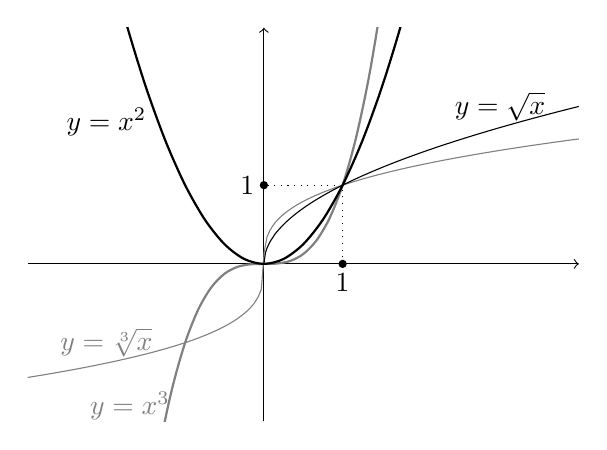
\begin{tikzpicture}[x=1.0cm,y=1.0cm]
      \clip(-3,-2) rectangle (4,3);
    	\draw[->] (-3,0) -- (4,0);
      \draw[->] (0,-2) -- (0,3);
      \draw[dotted] (1,0) -- (1,1) -- (0,1);
%      \draw[domain=0.2:4,samples=50,variable=\x,dashed,color=gray] plot
%        ({\x}, {1/(\x))});
%      \draw[domain=-3:-0.5,samples=50,variable=\x,dashed,color=gray] plot
%        ({\x}, {1/(\x))});
      \draw[domain=-2.0:2.0,smooth,variable=\x,thick,color=gray] plot
        ({\x}, {\x*\x*\x)});
      \draw[domain=-3.1:4.0,samples=200,variable=\x,color=gray] plot
        ({\x}, {pow(abs(\x),1/3)*\x / abs(\x)});
      \draw[domain=-3.0:3.0,smooth,variable=\x,thick] plot
        ({\x}, {\x*\x});
      \draw[domain=0.0:4.0,samples=200,variable=\x] plot
      ({\x}, {pow(\x,1/2)});
      \node at (-2.0,1.8) {$y=x^2$};
      \node at (3,2) {$y=\sqrt{x}$};
      \node[color=gray] at (-1.7,-1.8) {$y=x^{3}$};
      \node[color=gray] at (-2.0,-1) {$y=\sqrt[3]{x}$};
      \fill (1,0) node[below]{$1$} circle[radius=1.5pt];
      \fill (0,1) node[left]{$1$} circle[radius=1.5pt];
    \end{tikzpicture}
  \end{center}
  \caption{Graphs of the powers $x^2$, $x^3$ and roots
  $\sqrt x$, $\sqrt[3] x$.}
  \label{fig:potenza_intera_radice}
\end{figure}

%\subsubsection{irrational numbers}
%
%
%We have thus demonstrated that $\QQ$ cannot be continuous (otherwise it would be isomorphic to $\RR$ where the equation $x^2=2$ has a solution). Using the irrationality of $\sqrt 2$, we can now exhibit an example of subsets of $\QQ$ that are \emph{separated} (in the sense of definition~\ref{def:ordinamento_continuo}) but do not have a separation element in $\QQ$:
%\[
%A= \ENCLOSE{x\in\QQ\colon x^2< 2},
%\qquad
%B = \ENCLOSE{x\in \QQ\colon x<0, x^2>2}.  
%\]
%Clearly, $A\le B$, but in $\RR$, these two sets have as their only separation element $\sqrt 2$, which is not